\documentclass[11pt]{report}
\renewcommand{\baselinestretch}{1.5}


% Declaração dos pacotes
\usepackage[utf8]{inputenc}
\usepackage[T1]{fontenc}
\usepackage{graphicx}
\usepackage[portuguese]{babel}
\usepackage{graphicx}
\usepackage[affil-it]{authblk} % Usado para meter nome da escola
\usepackage{eurosym} % Usado para o €
\usepackage{url} % URL



% CAPA
\title{\textbf{\textit{Exploração e desenvolvimento  de processos de interoperabilidade entre sistemas, assentes em serviços web.}\\
		\large2º Trabalho prático de
		Integração de Sistemas de Informação}}
			
				
\author{Rúben Guimarães nº11156}

\affil{Escola Superior de Tecnologia, IPCA \\
	Barcelos}	
	
		
\date{10 de Novembro de 2017}


\begin{document}

\maketitle




% Indice
\tableofcontents


% Introdução
\chapter*{Introdução}
\addcontentsline{toc}{chapter}{Introdução}

O trabalho prático abordado neste relatório foi desenvolvido no âmbito da unidade curricular Integração de Sistemas de Informação do curso de Engenharia de Sistemas Informáticos, lecionada pelo docente Luís Ferreira. O docente desafiou os alunos a criar um projeto que aplicasse e experimenta-se serviços SOAP e RESTful, complementada com a utilização de serviços externos existentes.

\clearpage



% Resumo
\chapter*{Resumo}
\addcontentsline{toc}{chapter}{Resumo}

Neste trabalho desenvolvi um pequeno serviço que é alojado na platforma Azure que é uma solução para alojamento de serviços e aplicações na \textit{cloud}. 
Este serviço recorre a 4 API's externas para receber informação sobre o endereço IP da nossa ligação ou de uma fornecida, para recolher informação metereologica de uma dada cidade e por fim para publicar um \textit{Tweet} no \textit{Twitter} ou para publicar a informação metereologica da cidade consultada no \textit{Twitter}.\\ Por fim desenvolvi recorrendo ao \textit{Windows Presentation Foundation} (WPF) que recorre a linguagem de marcação \textit{Extensible Application Markup Language} (XAML) um cliente que utiliza os serviços desenvolvidos.

\clearpage


% Objectivos
\chapter*{Objectivos}
\addcontentsline{toc}{chapter}{Objectivos}

Os objetivos que defini para o meu projeto foram os seguintes:

\begin{itemize}
\item Usar uma API externa para saber o endereço IP da minha ligação.
\item Usar uma API externa para saber informação sobre um endereço IP.
\item Usar uma API externa para publicar \textit{Tweets} no \textit{Twitter}.
\item Usar uma API externa para receber informação metereologica de uma cidade.
\item Controlar a execução de serviços com recurso a credencias de autenticação (protocolo OAuth).
\item Publicar o serviço na platforma Azure.
\item Publicar e usar uma base da dados na platforma Azure.
\item Desevolvimento de um cliente que utilize os serviços desevolvidos.
\item Diversos tipo de operações CRUD recorrendo aos serviços RESTful.
\item Utilização de um sistema de controlo de versões no desevolvimento (GIT).
\end{itemize}


\clearpage


% Arquitectura
\chapter*{Arquitectura}
\addcontentsline{toc}{chapter}{Arquitectura}

Podemos consultar na figura seguinte um diagrama com a arquitectura do projecto.

\begin{figure} [!h]
\centering
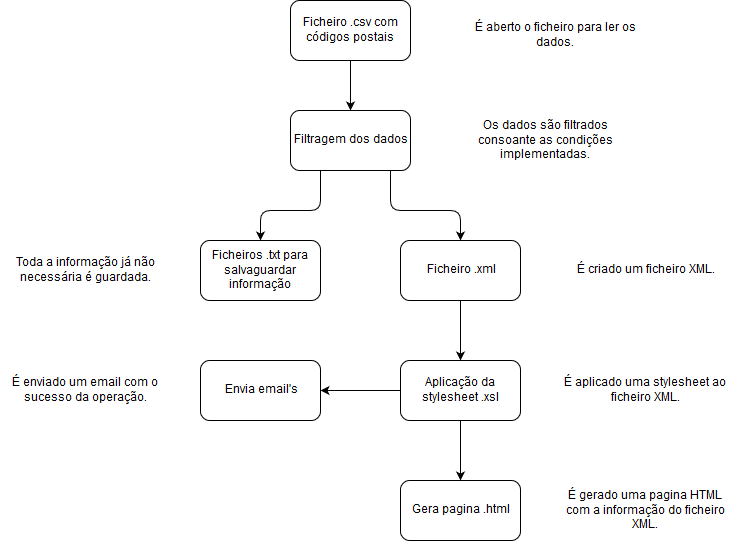
\includegraphics[width=\textwidth]{Prints_Trabalho/diagrama.png}
\caption{Diagrama da arquitectura do projecto}
\label{Rotulo}
\end{figure}


\clearpage


% Recursos usados no projecto
\chapter*{Recursos usados no projecto}
\addcontentsline{toc}{chapter}{Recursos usados no projecto}

Para o desenvolvimento do projecto foram utilizados os seguintes recursos:

\textbf{Software:}
\begin{itemize}
\item \textit{Visual Studio 2017} para o desevolvimento do cliente e do serviço.
\item \textit{Microsoft SQL Server Management 2017} para o criação de tabelas na base de dados.
\item \textit{Firefox Quantum 57.0.4} para teste dos serviços criados.
\end{itemize}

\textbf{Outros:}
\begin{itemize}
\item \textit{json2csharp} para a criação de classes dos ficheiros \textit{JSON}. \cite{json2csharp}
\item \textit{TinyTwitter} usada para facilitar a comunicação com o \textit{Twitter}.\cite{TinyTwitter}
\item \textit{Azure} usado para alojar o serviço e base de dados. \cite{TinyTwitter}
\end{itemize}



% API's externas usadas
\chapter*{API's externas usadas}
\addcontentsline{toc}{chapter}{API's externas usadas}

Foram usadas 4 API's externas:

\begin{itemize}
\item \textit{ipapi.co} - Usada para receber um ficheiro \textit{JSON} com as informações de um dado endereço IP.\cite{ipapi}
\item \textit{ipify  A  Simple IP Address API} - Usada para receber uma string com o endereço IP da nossa ligação.\cite{ipify}
\item \textit{Twitter Developer Platform} - Usada para publicar\textit{Tweets}  no \textit{Twitter}. \cite{twitter}
\item \textit{OpenWeatherMap} - Usada para receber um ficheiro \textit{JSON} com a informação meteologica de uma dada cidade. \cite{Weather}
\end{itemize}


% Desenvolvimento
\chapter*{Desenvolvimento}
\addcontentsline{toc}{chapter}{Desenvolvimento}

O serviço foi desenvolvido recorrendo a um serviço do tipo \textit{Windows Communication Foundation} (WCF). Este efetua a comunicação com as API's externas, trabalha os dados recebidos (se necessário) e disponibiliza serviços para um ou mais cliente usarem. Os serviços que disponibiliza são os seguintes:
\begin{itemize}
\item \textbf{GetIPInfo/\{enderecoIP\}} do tipo GET que envia a informação do endereço IP recebido no campo enderecoIP, num ficheiro \textit{JSON}
\item \textbf{MyIp} do tipo GET que envia a informação do endereço IP da ligação numa string.
\item \textbf{Tweet} do tipo POST que receber uma mensagem e publicar essa mensagem na conta \url{https://twitter.com/trabalhoisi}. Este recorre a uma biblioteca\cite{TinyTwitter} para facilitar a comunicação com o \textit{Twitter}.
\item \textbf{Weather/\{nomeCidade\}} do tipo GET que envia a informação metereologica da cidade recebida  no campo nomeCidade, num ficheiro \textit{JSON}
\end{itemize}

\clearpage

O serviço também contem objectos para guardar as respostas recebidas em \textit{JSON} criados no serviço \textit{json2csharp} tal como podemos verificar na imagem seguinte:

\begin{figure} [!h]
\centering
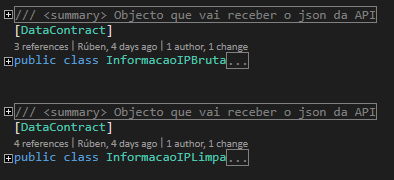
\includegraphics[width=\textwidth]{Prints_Trabalho/objectos.png}
\caption{Objectos \textit{JSON}}
\label{Rotulo}
\end{figure}

Este serviço atualmente esta publicado no \textit{Azure} e pode ser chamado usando o seguinte link \url{http://wcfrest20180109101801.azurewebsites.net/Service.svc/}.

\clearpage

O cliente foi  desenvolvido recorrendo ao \textit{Windows Presentation Foundation} (WPF) que recorre a linguagem de marcação \textit{Extensible Application Markup Language} (XAML) . Este é composto por 3 ambas (Endereços de IP/ Twitter / Meteorologia) onde existe uma interface onde podemos testar os serviços desevolvidos e ver os resultados. Podemos ver a aba do \textit{Twitter} na imagem seguinte.

\begin{figure} [!h]
\centering
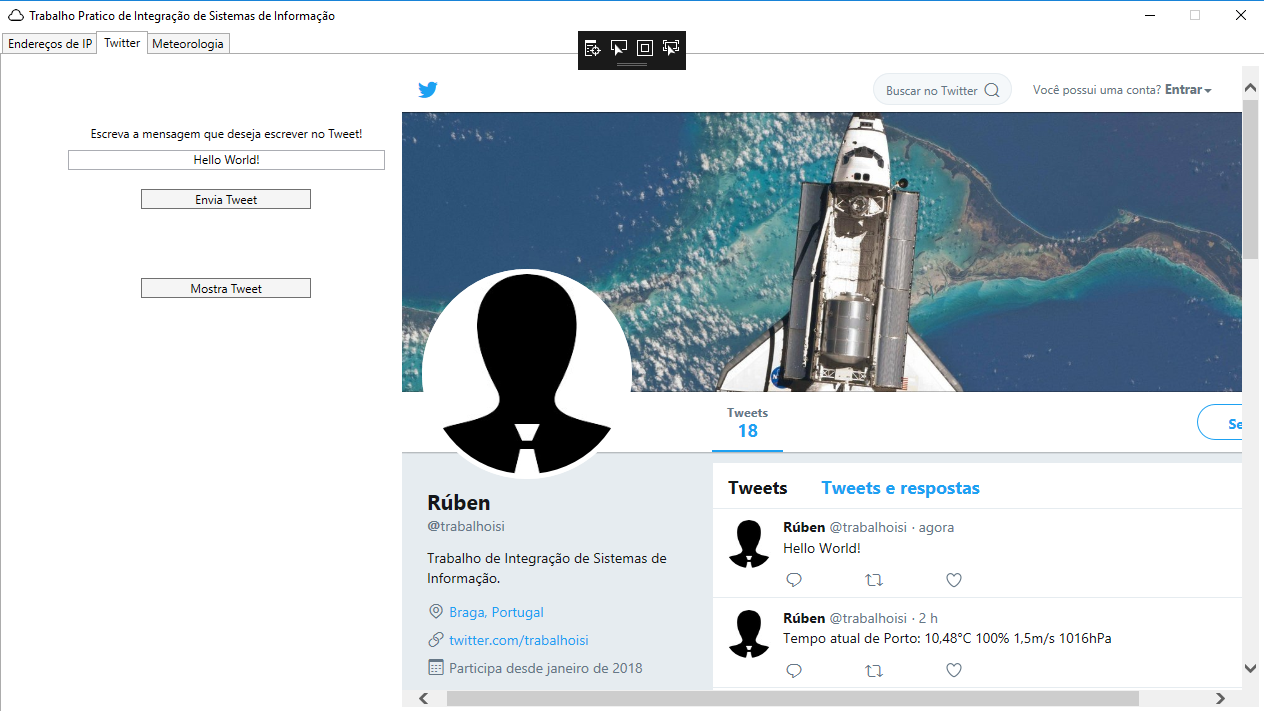
\includegraphics[width=\textwidth]{Prints_Trabalho/cliente.png}
\caption{Cliente desenvolvido}
\label{Rotulo}
\end{figure}


% Conclução
\chapter*{Conclusão}
\addcontentsline{toc}{chapter}{Conclusão}

Este trabalho permitiu-se aplicar os conhecimentos adquiridos durante o desenrolar da unidade curricular de Integração de Sistemas de Informação e explorar e desenvolver processos de interoperabilidade entre sistemas, assentes em serviços web. Uma das partes que correu mal no trabalho foi o uso da base de dados alojada no \textit{Azure} que por algum motivo não mantinha a ligação aberta quando a tentava usar no serviço. De qualquer forma acho que este trabalho foi um sucesso tendo conseguido alcançar os meus objetivos e ficando a conheçer mais sobre serviços RESTful.

% Bilbiografia
\begin{thebibliography}{2}

	\bibitem{json2csharp}
	\emph{json2csharp }.  01 Janeiro, 2018. 
	\url{http://json2csharp.com/}


	\bibitem{TinyTwitter}
	jmhdez. \emph{TinyTwitter}.  01 Janeiro, 2018. 
	\url{https://github.com/jmhdez/TinyTwitter}


	\bibitem{Azure}
	\emph{Azure}.  01 Janeiro, 2018. 
	\url{https://portal.azure.com/}


	\bibitem{ipapi}
	\emph{ipapi.co}.  01 Janeiro, 2018. 
	\url{https://ipapi.co/}


	\bibitem{ipify}
	\emph{ipify} A Simple IP Address API.  01 Janeiro, 2018. 
	\url{https://www.ipify.org/}


	\bibitem{twitter}
	\emph{Twitter} Developer Platform.  03 Janeiro, 2018. 
	\url{https://developer.twitter.com/}


	\bibitem{Weather}
	\emph{OpenWeatherMap} Current weather and forecasts in your city.  05 Janeiro, 2018. 
	\url{http://openweathermap.org/current}
	

\end{thebibliography}
\addcontentsline{toc}{chapter}{Bibliografia}

\end{document}